\documentclass[1p]{elsarticle_modified}
%\bibliographystyle{elsarticle-num}

%\usepackage[colorlinks]{hyperref}
%\usepackage{abbrmath_seonhwa} %\Abb, \Ascr, \Acal ,\Abf, \Afrak
\usepackage{amsfonts}
\usepackage{amssymb}
\usepackage{amsmath}
\usepackage{amsthm}
\usepackage{scalefnt}
\usepackage{amsbsy}
\usepackage{kotex}
\usepackage{caption}
\usepackage{subfig}
\usepackage{color}
\usepackage{graphicx}
\usepackage{xcolor} %% white, black, red, green, blue, cyan, magenta, yellow
\usepackage{float}
\usepackage{setspace}
\usepackage{hyperref}

\usepackage{tikz}
\usetikzlibrary{arrows}

\usepackage{multirow}
\usepackage{array} % fixed length table
\usepackage{hhline}

%%%%%%%%%%%%%%%%%%%%%
\makeatletter
\renewcommand*\env@matrix[1][\arraystretch]{%
	\edef\arraystretch{#1}%
	\hskip -\arraycolsep
	\let\@ifnextchar\new@ifnextchar
	\array{*\c@MaxMatrixCols c}}
\makeatother %https://tex.stackexchange.com/questions/14071/how-can-i-increase-the-line-spacing-in-a-matrix
%%%%%%%%%%%%%%%

\usepackage[normalem]{ulem}

\newcommand{\msout}[1]{\ifmmode\text{\sout{\ensuremath{#1}}}\else\sout{#1}\fi}
%SOURCE: \msout is \stkout macro in https://tex.stackexchange.com/questions/20609/strikeout-in-math-mode

\newcommand{\cancel}[1]{
	\ifmmode
	{\color{red}\msout{#1}}
	\else
	{\color{red}\sout{#1}}
	\fi
}

\newcommand{\add}[1]{
	{\color{blue}\uwave{#1}}
}

\newcommand{\replace}[2]{
	\ifmmode
	{\color{red}\msout{#1}}{\color{blue}\uwave{#2}}
	\else
	{\color{red}\sout{#1}}{\color{blue}\uwave{#2}}
	\fi
}

\newcommand{\Sol}{\mathcal{S}} %segment
\newcommand{\D}{D} %diagram
\newcommand{\A}{\mathcal{A}} %arc


%%%%%%%%%%%%%%%%%%%%%%%%%%%%%5 test

\def\sl{\operatorname{\textup{SL}}(2,\Cbb)}
\def\psl{\operatorname{\textup{PSL}}(2,\Cbb)}
\def\quan{\mkern 1mu \triangleright \mkern 1mu}

\theoremstyle{definition}
\newtheorem{thm}{Theorem}[section]
\newtheorem{prop}[thm]{Proposition}
\newtheorem{lem}[thm]{Lemma}
\newtheorem{ques}[thm]{Question}
\newtheorem{cor}[thm]{Corollary}
\newtheorem{defn}[thm]{Definition}
\newtheorem{exam}[thm]{Example}
\newtheorem{rmk}[thm]{Remark}
\newtheorem{alg}[thm]{Algorithm}

\newcommand{\I}{\sqrt{-1}}
\begin{document}

%\begin{frontmatter}
%
%\title{Boundary parabolic representations of knots up to 8 crossings}
%
%%% Group authors per affiliation:
%\author{Yunhi Cho} 
%\address{Department of Mathematics, University of Seoul, Seoul, Korea}
%\ead{yhcho@uos.ac.kr}
%
%
%\author{Seonhwa Kim} %\fnref{s_kim}}
%\address{Center for Geometry and Physics, Institute for Basic Science, Pohang, 37673, Korea}
%\ead{ryeona17@ibs.re.kr}
%
%\author{Hyuk Kim}
%\address{Department of Mathematical Sciences, Seoul National University, Seoul 08826, Korea}
%\ead{hyukkim@snu.ac.kr}
%
%\author{Seokbeom Yoon}
%\address{Department of Mathematical Sciences, Seoul National University, Seoul, 08826,  Korea}
%\ead{sbyoon15@snu.ac.kr}
%
%\begin{abstract}
%We find all boundary parabolic representation of knots up to 8 crossings.
%
%\end{abstract}
%\begin{keyword}
%    \MSC[2010] 57M25 
%\end{keyword}
%
%\end{frontmatter}

%\linenumbers
%\tableofcontents
%
\newcommand\colored[1]{\textcolor{white}{\rule[-0.35ex]{0.8em}{1.4ex}}\kern-0.8em\color{red} #1}%
%\newcommand\colored[1]{\textcolor{white}{ #1}\kern-2.17ex	\textcolor{white}{ #1}\kern-1.81ex	\textcolor{white}{ #1}\kern-2.15ex\color{red}#1	}

{\Large $\underline{12n_{0841}~(K12n_{0841})}$}

\setlength{\tabcolsep}{10pt}
\renewcommand{\arraystretch}{1.6}
\vspace{1cm}\begin{tabular}{m{100pt}>{\centering\arraybackslash}m{274pt}}
\multirow{5}{120pt}{
	\centering
	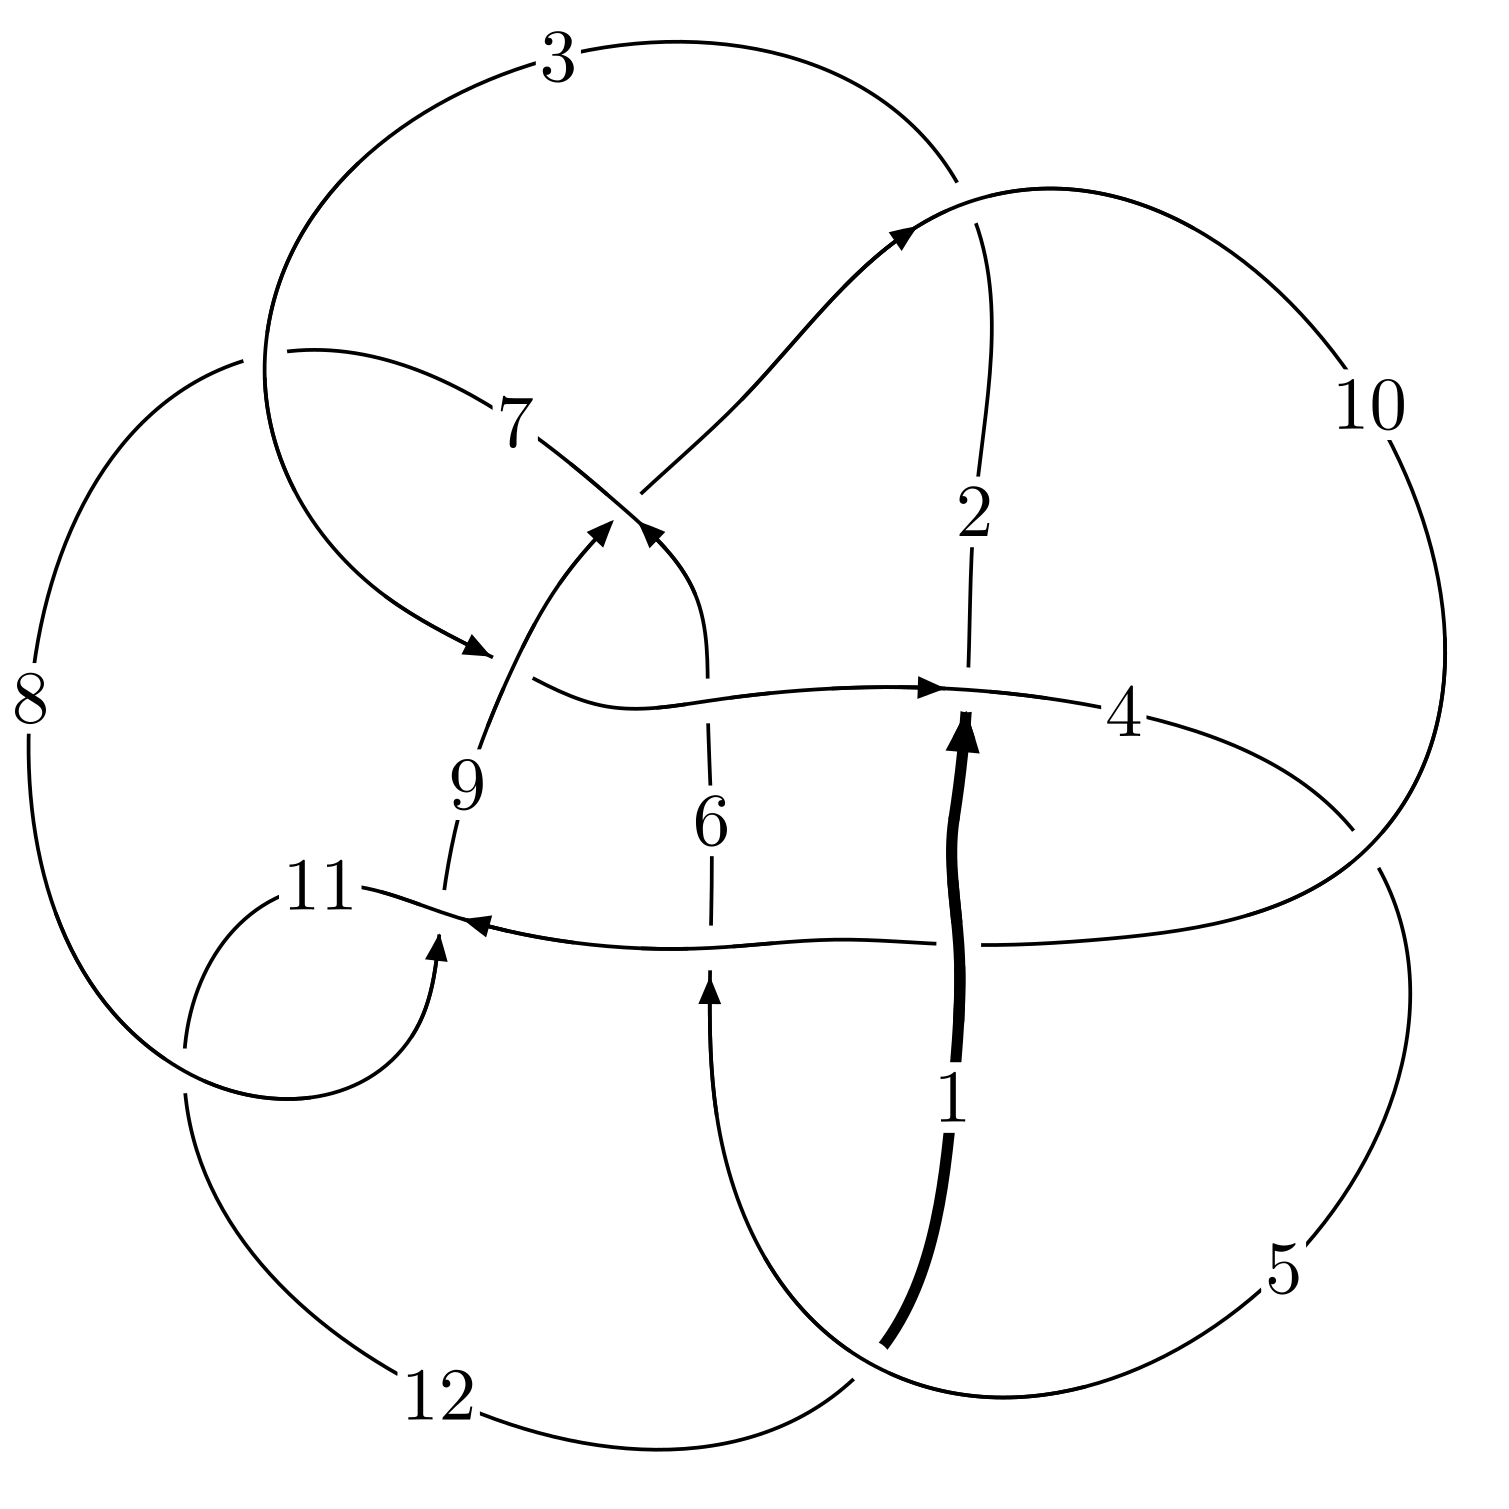
\includegraphics[width=112pt]{../../../GIT/diagram.site/Diagrams/png/2930_12n_0841.png}\\
\ \ \ A knot diagram\footnotemark}&
\allowdisplaybreaks
\textbf{Linearized knot diagam} \\
\cline{2-2}
 &
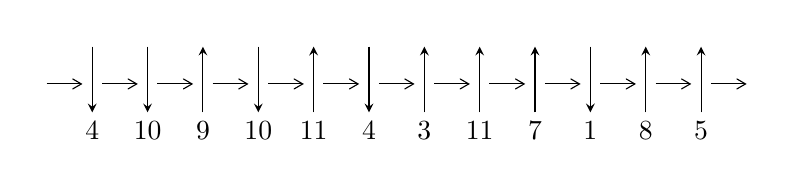
\begin{tikzpicture}[x=20pt, y=17pt]
	% nodes
	\node (C0) at (0, 0) {};
	\node (C1) at (1, 0) {};
	\node (C1U) at (1, +1) {};
	\node (C1D) at (1, -1) {4};

	\node (C2) at (2, 0) {};
	\node (C2U) at (2, +1) {};
	\node (C2D) at (2, -1) {10};

	\node (C3) at (3, 0) {};
	\node (C3U) at (3, +1) {};
	\node (C3D) at (3, -1) {9};

	\node (C4) at (4, 0) {};
	\node (C4U) at (4, +1) {};
	\node (C4D) at (4, -1) {10};

	\node (C5) at (5, 0) {};
	\node (C5U) at (5, +1) {};
	\node (C5D) at (5, -1) {11};

	\node (C6) at (6, 0) {};
	\node (C6U) at (6, +1) {};
	\node (C6D) at (6, -1) {4};

	\node (C7) at (7, 0) {};
	\node (C7U) at (7, +1) {};
	\node (C7D) at (7, -1) {3};

	\node (C8) at (8, 0) {};
	\node (C8U) at (8, +1) {};
	\node (C8D) at (8, -1) {11};

	\node (C9) at (9, 0) {};
	\node (C9U) at (9, +1) {};
	\node (C9D) at (9, -1) {7};

	\node (C10) at (10, 0) {};
	\node (C10U) at (10, +1) {};
	\node (C10D) at (10, -1) {1};

	\node (C11) at (11, 0) {};
	\node (C11U) at (11, +1) {};
	\node (C11D) at (11, -1) {8};

	\node (C12) at (12, 0) {};
	\node (C12U) at (12, +1) {};
	\node (C12D) at (12, -1) {5};
	\node (C13) at (13, 0) {};

	% arrows
	\draw[->,>={angle 60}]
	(C0) edge (C1) (C1) edge (C2) (C2) edge (C3) (C3) edge (C4) (C4) edge (C5) (C5) edge (C6) (C6) edge (C7) (C7) edge (C8) (C8) edge (C9) (C9) edge (C10) (C10) edge (C11) (C11) edge (C12) (C12) edge (C13) ;	\draw[->,>=stealth]
	(C1U) edge (C1D) (C2U) edge (C2D) (C3D) edge (C3U) (C4U) edge (C4D) (C5D) edge (C5U) (C6U) edge (C6D) (C7D) edge (C7U) (C8D) edge (C8U) (C9D) edge (C9U) (C10U) edge (C10D) (C11D) edge (C11U) (C12D) edge (C12U) ;
	\end{tikzpicture} \\
\hhline{~~} \\& 
\textbf{Solving Sequence} \\ \cline{2-2} 
 &
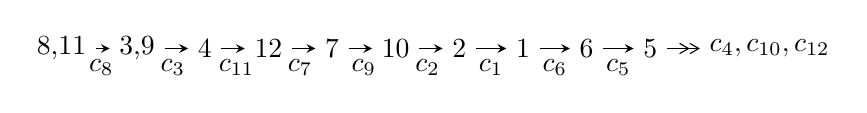
\begin{tikzpicture}[x=23pt, y=7pt]
	% node
	\node (A0) at (-1/8, 0) {8,11};
	\node (A1) at (17/16, 0) {3,9};
	\node (A2) at (17/8, 0) {4};
	\node (A3) at (25/8, 0) {12};
	\node (A4) at (33/8, 0) {7};
	\node (A5) at (41/8, 0) {10};
	\node (A6) at (49/8, 0) {2};
	\node (A7) at (57/8, 0) {1};
	\node (A8) at (65/8, 0) {6};
	\node (A9) at (73/8, 0) {5};
	\node (C1) at (1/2, -1) {$c_{8}$};
	\node (C2) at (13/8, -1) {$c_{3}$};
	\node (C3) at (21/8, -1) {$c_{11}$};
	\node (C4) at (29/8, -1) {$c_{7}$};
	\node (C5) at (37/8, -1) {$c_{9}$};
	\node (C6) at (45/8, -1) {$c_{2}$};
	\node (C7) at (53/8, -1) {$c_{1}$};
	\node (C8) at (61/8, -1) {$c_{6}$};
	\node (C9) at (69/8, -1) {$c_{5}$};
	\node (A10) at (11, 0) {$c_{4},c_{10},c_{12}$};

	% edge
	\draw[->,>=stealth]	
	(A0) edge (A1) (A1) edge (A2) (A2) edge (A3) (A3) edge (A4) (A4) edge (A5) (A5) edge (A6) (A6) edge (A7) (A7) edge (A8) (A8) edge (A9) ;
	\draw[->>,>={angle 60}]	
	(A9) edge (A10);
\end{tikzpicture} \\ 

\end{tabular} \\

\footnotetext{
The image of knot diagram is generated by the software ``\textbf{Draw programme}" developed by Andrew Bartholomew(\url{http://www.layer8.co.uk/maths/draw/index.htm\#Running-draw}), where we modified some parts for our purpose(\url{https://github.com/CATsTAILs/LinksPainter}).
}\phantom \\ \newline 
\centering \textbf{Ideals for irreducible components\footnotemark of $X_{\text{par}}$} 
 
\begin{align*}
I^u_{1}&=\langle 
1.90108\times10^{282} u^{72}-2.46888\times10^{282} u^{71}+\cdots+1.59427\times10^{284} b-3.09209\times10^{284},\\
\phantom{I^u_{1}}&\phantom{= \langle  }-4.97935\times10^{284} u^{72}+5.96759\times10^{284} u^{71}+\cdots+6.85537\times10^{285} a+1.28477\times10^{286},\\
\phantom{I^u_{1}}&\phantom{= \langle  }u^{73}- u^{72}+\cdots-309 u-43\rangle \\
I^u_{2}&=\langle 
1.37214\times10^{26} u^{32}+1.11140\times10^{24} u^{31}+\cdots+5.91097\times10^{25} b-2.90680\times10^{26},\\
\phantom{I^u_{2}}&\phantom{= \langle  }6.79162\times10^{26} u^{32}+1.40659\times10^{27} u^{31}+\cdots+5.91097\times10^{25} a+1.02213\times10^{27},\;u^{33}+2 u^{32}+\cdots+u+1\rangle \\
\\
\end{align*}
\raggedright * 2 irreducible components of $\dim_{\mathbb{C}}=0$, with total 106 representations.\\
\footnotetext{All coefficients of polynomials are rational numbers. But the coefficients are sometimes approximated in decimal forms when there is not enough margin.}
\newpage
\renewcommand{\arraystretch}{1}
\centering \section*{I. $I^u_{1}= \langle 1.90\times10^{282} u^{72}-2.47\times10^{282} u^{71}+\cdots+1.59\times10^{284} b-3.09\times10^{284},\;-4.98\times10^{284} u^{72}+5.97\times10^{284} u^{71}+\cdots+6.86\times10^{285} a+1.28\times10^{286},\;u^{73}- u^{72}+\cdots-309 u-43 \rangle$}
\flushleft \textbf{(i) Arc colorings}\\
\begin{tabular}{m{7pt} m{180pt} m{7pt} m{180pt} }
\flushright $a_{8}=$&$\begin{pmatrix}1\\0\end{pmatrix}$ \\
\flushright $a_{11}=$&$\begin{pmatrix}0\\u\end{pmatrix}$ \\
\flushright $a_{3}=$&$\begin{pmatrix}0.0726344 u^{72}-0.0870499 u^{71}+\cdots-12.0464 u-1.87411\\-0.0119244 u^{72}+0.0154860 u^{71}+\cdots+4.04662 u+1.93950\end{pmatrix}$ \\
\flushright $a_{9}=$&$\begin{pmatrix}1\\- u^2\end{pmatrix}$ \\
\flushright $a_{4}=$&$\begin{pmatrix}0.0634815 u^{72}-0.0752458 u^{71}+\cdots-9.33095 u-0.554483\\-0.0114519 u^{72}+0.0149796 u^{71}+\cdots+3.62096 u+1.82549\end{pmatrix}$ \\
\flushright $a_{12}=$&$\begin{pmatrix}u\\u\end{pmatrix}$ \\
\flushright $a_{7}=$&$\begin{pmatrix}-0.0358045 u^{72}+0.0472121 u^{71}+\cdots-5.21020 u+16.8882\\-0.00222320 u^{72}+0.00250582 u^{71}+\cdots-2.28998 u+0.112053\end{pmatrix}$ \\
\flushright $a_{10}=$&$\begin{pmatrix}0.0845588 u^{72}-0.102536 u^{71}+\cdots-16.0931 u-3.81361\\-0.00645912 u^{72}+0.00933863 u^{71}+\cdots+0.00294395 u+1.06814\end{pmatrix}$ \\
\flushright $a_{2}=$&$\begin{pmatrix}0.158202 u^{72}-0.190926 u^{71}+\cdots-53.4190 u-2.27997\\-0.0208591 u^{72}+0.0252457 u^{71}+\cdots+6.05259 u+4.49812\end{pmatrix}$ \\
\flushright $a_{1}=$&$\begin{pmatrix}-0.00258344 u^{72}-0.00120206 u^{71}+\cdots+32.9271 u+6.85728\\-0.00790244 u^{72}+0.00893571 u^{71}+\cdots+7.42915 u+1.73646\end{pmatrix}$ \\
\flushright $a_{6}=$&$\begin{pmatrix}-0.0675535 u^{72}+0.0804100 u^{71}+\cdots+32.6859 u+7.80933\\0.00236218 u^{72}-0.00404640 u^{71}+\cdots+2.31253 u-0.239928\end{pmatrix}$ \\
\flushright $a_{5}=$&$\begin{pmatrix}-0.0675535 u^{72}+0.0804100 u^{71}+\cdots+32.6859 u+7.80933\\1.32859\times10^{-6} u^{72}-0.00128498 u^{71}+\cdots+3.38038 u+0.312900\end{pmatrix}$\\&\end{tabular}
\flushleft \textbf{(ii) Obstruction class $= -1$}\\~\\
\flushleft \textbf{(iii) Cusp Shapes $= 0.0794662 u^{72}-0.103769 u^{71}+\cdots-34.4075 u-13.9361$}\\~\\
\newpage\renewcommand{\arraystretch}{1}
\flushleft \textbf{(iv) u-Polynomials at the component}\newline \\
\begin{tabular}{m{50pt}|m{274pt}}
Crossings & \hspace{64pt}u-Polynomials at each crossing \\
\hline $$\begin{aligned}c_{1}\end{aligned}$$&$\begin{aligned}
&u^{73}+6 u^{72}+\cdots-63093 u-11592
\end{aligned}$\\
\hline $$\begin{aligned}c_{2}\end{aligned}$$&$\begin{aligned}
&u^{73}+3 u^{72}+\cdots+20760218389 u+1628977223
\end{aligned}$\\
\hline $$\begin{aligned}c_{3}\end{aligned}$$&$\begin{aligned}
&u^{73}+u^{72}+\cdots+56046 u-10579
\end{aligned}$\\
\hline $$\begin{aligned}c_{4}\end{aligned}$$&$\begin{aligned}
&u^{73}-2 u^{72}+\cdots+285527 u-23711
\end{aligned}$\\
\hline $$\begin{aligned}c_{5}\end{aligned}$$&$\begin{aligned}
&u^{73}+46 u^{71}+\cdots+172232704 u-28909568
\end{aligned}$\\
\hline $$\begin{aligned}c_{6}\end{aligned}$$&$\begin{aligned}
&u^{73}-8 u^{72}+\cdots+26606 u+4801
\end{aligned}$\\
\hline $$\begin{aligned}c_{7}\end{aligned}$$&$\begin{aligned}
&u^{73}-5 u^{72}+\cdots-1326094 u-293207
\end{aligned}$\\
\hline $$\begin{aligned}c_{8},c_{11}\end{aligned}$$&$\begin{aligned}
&u^{73}- u^{72}+\cdots-309 u-43
\end{aligned}$\\
\hline $$\begin{aligned}c_{9}\end{aligned}$$&$\begin{aligned}
&u^{73}+4 u^{72}+\cdots-19 u-4
\end{aligned}$\\
\hline $$\begin{aligned}c_{10}\end{aligned}$$&$\begin{aligned}
&u^{73}-5 u^{72}+\cdots+9 u-1
\end{aligned}$\\
\hline $$\begin{aligned}c_{12}\end{aligned}$$&$\begin{aligned}
&u^{73}+45 u^{71}+\cdots+241471 u+54913
\end{aligned}$\\
\hline
\end{tabular}\\~\\
\newpage\renewcommand{\arraystretch}{1}
\flushleft \textbf{(v) Riley Polynomials at the component}\newline \\
\begin{tabular}{m{50pt}|m{274pt}}
Crossings & \hspace{64pt}Riley Polynomials at each crossing \\
\hline $$\begin{aligned}c_{1}\end{aligned}$$&$\begin{aligned}
&y^{73}-88 y^{72}+\cdots+7315837785 y-134374464
\end{aligned}$\\
\hline $$\begin{aligned}c_{2}\end{aligned}$$&$\begin{aligned}
&y^{73}-75 y^{72}+\cdots+5.45\times10^{20} y-2.65\times10^{18}
\end{aligned}$\\
\hline $$\begin{aligned}c_{3}\end{aligned}$$&$\begin{aligned}
&y^{73}+25 y^{72}+\cdots-491484062 y-111915241
\end{aligned}$\\
\hline $$\begin{aligned}c_{4}\end{aligned}$$&$\begin{aligned}
&y^{73}-82 y^{72}+\cdots+5333119705 y-562211521
\end{aligned}$\\
\hline $$\begin{aligned}c_{5}\end{aligned}$$&$\begin{aligned}
&y^{73}+92 y^{72}+\cdots-5265299779616768 y-835763121946624
\end{aligned}$\\
\hline $$\begin{aligned}c_{6}\end{aligned}$$&$\begin{aligned}
&y^{73}-52 y^{72}+\cdots-10859270 y-23049601
\end{aligned}$\\
\hline $$\begin{aligned}c_{7}\end{aligned}$$&$\begin{aligned}
&y^{73}+29 y^{72}+\cdots-2637873238424 y-85970344849
\end{aligned}$\\
\hline $$\begin{aligned}c_{8},c_{11}\end{aligned}$$&$\begin{aligned}
&y^{73}+65 y^{72}+\cdots-4365 y-1849
\end{aligned}$\\
\hline $$\begin{aligned}c_{9}\end{aligned}$$&$\begin{aligned}
&y^{73}+4 y^{72}+\cdots-343 y-16
\end{aligned}$\\
\hline $$\begin{aligned}c_{10}\end{aligned}$$&$\begin{aligned}
&y^{73}+3 y^{72}+\cdots-49 y-1
\end{aligned}$\\
\hline $$\begin{aligned}c_{12}\end{aligned}$$&$\begin{aligned}
&y^{73}+90 y^{72}+\cdots+125937776729 y-3015437569
\end{aligned}$\\
\hline
\end{tabular}\\~\\
\newpage\flushleft \textbf{(vi) Complex Volumes and Cusp Shapes}
$$\begin{array}{c|c|c}  
\text{Solutions to }I^u_{1}& \I (\text{vol} + \sqrt{-1}CS) & \text{Cusp shape}\\
 \hline 
\begin{aligned}
u &= -0.127388 + 1.019780 I \\
a &= -0.27880 + 2.25156 I \\
b &= -0.420810 + 1.154600 I\end{aligned}
 & -5.96688 + 0.04720 I & \phantom{-0.000000 } 0 \\ \hline\begin{aligned}
u &= -0.127388 - 1.019780 I \\
a &= -0.27880 - 2.25156 I \\
b &= -0.420810 - 1.154600 I\end{aligned}
 & -5.96688 - 0.04720 I & \phantom{-0.000000 } 0 \\ \hline\begin{aligned}
u &= -0.546347 + 0.885676 I \\
a &= -1.43696 - 0.50950 I \\
b &= -0.485548 - 1.108380 I\end{aligned}
 & -3.59850 - 4.60468 I & \phantom{-0.000000 } 0 \\ \hline\begin{aligned}
u &= -0.546347 - 0.885676 I \\
a &= -1.43696 + 0.50950 I \\
b &= -0.485548 + 1.108380 I\end{aligned}
 & -3.59850 + 4.60468 I & \phantom{-0.000000 } 0 \\ \hline\begin{aligned}
u &= \phantom{-}0.957502\phantom{ +0.000000I} \\
a &= \phantom{-}0.139905\phantom{ +0.000000I} \\
b &= \phantom{-}0.588088\phantom{ +0.000000I}\end{aligned}
 & \phantom{-}1.55339\phantom{ +0.000000I} & \phantom{-0.000000 } 0 \\ \hline\begin{aligned}
u &= \phantom{-}0.753002 + 0.520273 I \\
a &= \phantom{-}0.432133 + 0.644140 I \\
b &= -0.507710 + 0.528497 I\end{aligned}
 & \phantom{-}0.328053 + 1.143710 I & \phantom{-0.000000 } 0 \\ \hline\begin{aligned}
u &= \phantom{-}0.753002 - 0.520273 I \\
a &= \phantom{-}0.432133 - 0.644140 I \\
b &= -0.507710 - 0.528497 I\end{aligned}
 & \phantom{-}0.328053 - 1.143710 I & \phantom{-0.000000 } 0 \\ \hline\begin{aligned}
u &= \phantom{-}0.553850 + 1.039870 I \\
a &= \phantom{-}0.808148 - 0.733469 I \\
b &= -0.335070 - 0.338007 I\end{aligned}
 & -0.05050 + 2.22046 I & \phantom{-0.000000 } 0 \\ \hline\begin{aligned}
u &= \phantom{-}0.553850 - 1.039870 I \\
a &= \phantom{-}0.808148 + 0.733469 I \\
b &= -0.335070 + 0.338007 I\end{aligned}
 & -0.05050 - 2.22046 I & \phantom{-0.000000 } 0 \\ \hline\begin{aligned}
u &= \phantom{-}0.038876 + 1.186330 I \\
a &= \phantom{-}0.49937 + 1.40132 I \\
b &= \phantom{-}0.297313 + 0.986317 I\end{aligned}
 & -2.73445 + 2.20929 I & \phantom{-0.000000 } 0\\
 \hline 
 \end{array}$$\newpage$$\begin{array}{c|c|c}  
\text{Solutions to }I^u_{1}& \I (\text{vol} + \sqrt{-1}CS) & \text{Cusp shape}\\
 \hline 
\begin{aligned}
u &= \phantom{-}0.038876 - 1.186330 I \\
a &= \phantom{-}0.49937 - 1.40132 I \\
b &= \phantom{-}0.297313 - 0.986317 I\end{aligned}
 & -2.73445 - 2.20929 I & \phantom{-0.000000 } 0 \\ \hline\begin{aligned}
u &= \phantom{-}0.157164 + 1.238850 I \\
a &= \phantom{-}0.211536 + 1.345470 I \\
b &= \phantom{-}0.198177 + 1.356360 I\end{aligned}
 & -2.86036 + 2.78323 I & \phantom{-0.000000 } 0 \\ \hline\begin{aligned}
u &= \phantom{-}0.157164 - 1.238850 I \\
a &= \phantom{-}0.211536 - 1.345470 I \\
b &= \phantom{-}0.198177 - 1.356360 I\end{aligned}
 & -2.86036 - 2.78323 I & \phantom{-0.000000 } 0 \\ \hline\begin{aligned}
u &= \phantom{-}1.242360 + 0.227658 I \\
a &= \phantom{-}0.176398 - 0.372203 I \\
b &= \phantom{-}0.181626 - 0.479125 I\end{aligned}
 & \phantom{-}1.11769 + 1.51817 I & \phantom{-0.000000 } 0 \\ \hline\begin{aligned}
u &= \phantom{-}1.242360 - 0.227658 I \\
a &= \phantom{-}0.176398 + 0.372203 I \\
b &= \phantom{-}0.181626 + 0.479125 I\end{aligned}
 & \phantom{-}1.11769 - 1.51817 I & \phantom{-0.000000 } 0 \\ \hline\begin{aligned}
u &= -0.565862 + 0.457593 I \\
a &= \phantom{-}0.370741 - 0.432657 I \\
b &= \phantom{-}1.178140 + 0.731701 I\end{aligned}
 & \phantom{-}3.28841 + 2.32761 I & \phantom{-}7.74126 + 0.64227 I \\ \hline\begin{aligned}
u &= -0.565862 - 0.457593 I \\
a &= \phantom{-}0.370741 + 0.432657 I \\
b &= \phantom{-}1.178140 - 0.731701 I\end{aligned}
 & \phantom{-}3.28841 - 2.32761 I & \phantom{-}7.74126 - 0.64227 I \\ \hline\begin{aligned}
u &= -0.564181 + 1.141560 I \\
a &= -0.27712 - 1.76386 I \\
b &= \phantom{-}1.32972 - 1.19569 I\end{aligned}
 & \phantom{-}1.21585 - 6.81490 I & \phantom{-0.000000 } 0 \\ \hline\begin{aligned}
u &= -0.564181 - 1.141560 I \\
a &= -0.27712 + 1.76386 I \\
b &= \phantom{-}1.32972 + 1.19569 I\end{aligned}
 & \phantom{-}1.21585 + 6.81490 I & \phantom{-0.000000 } 0 \\ \hline\begin{aligned}
u &= \phantom{-}0.163845 + 1.294260 I \\
a &= -0.383545 + 1.220500 I \\
b &= -0.755460 + 1.149210 I\end{aligned}
 & -4.96510 + 3.26137 I & \phantom{-0.000000 } 0\\
 \hline 
 \end{array}$$\newpage$$\begin{array}{c|c|c}  
\text{Solutions to }I^u_{1}& \I (\text{vol} + \sqrt{-1}CS) & \text{Cusp shape}\\
 \hline 
\begin{aligned}
u &= \phantom{-}0.163845 - 1.294260 I \\
a &= -0.383545 - 1.220500 I \\
b &= -0.755460 - 1.149210 I\end{aligned}
 & -4.96510 - 3.26137 I & \phantom{-0.000000 } 0 \\ \hline\begin{aligned}
u &= -1.295820 + 0.293548 I \\
a &= -0.220803 + 0.150460 I \\
b &= \phantom{-}0.579096 - 0.311435 I\end{aligned}
 & \phantom{-}4.49917 - 3.40407 I & \phantom{-0.000000 } 0 \\ \hline\begin{aligned}
u &= -1.295820 - 0.293548 I \\
a &= -0.220803 - 0.150460 I \\
b &= \phantom{-}0.579096 + 0.311435 I\end{aligned}
 & \phantom{-}4.49917 + 3.40407 I & \phantom{-0.000000 } 0 \\ \hline\begin{aligned}
u &= -0.648670 + 0.020454 I \\
a &= \phantom{-}0.496880 - 0.830329 I \\
b &= -0.727089 - 0.500170 I\end{aligned}
 & -2.50658 + 2.13672 I & -1.93005 - 4.19239 I \\ \hline\begin{aligned}
u &= -0.648670 - 0.020454 I \\
a &= \phantom{-}0.496880 + 0.830329 I \\
b &= -0.727089 + 0.500170 I\end{aligned}
 & -2.50658 - 2.13672 I & -1.93005 + 4.19239 I \\ \hline\begin{aligned}
u &= \phantom{-}0.742224 + 1.151680 I \\
a &= \phantom{-}0.58786 - 1.48452 I \\
b &= -0.331175 - 1.062620 I\end{aligned}
 & -1.56569 + 4.54226 I & \phantom{-0.000000 } 0 \\ \hline\begin{aligned}
u &= \phantom{-}0.742224 - 1.151680 I \\
a &= \phantom{-}0.58786 + 1.48452 I \\
b &= -0.331175 + 1.062620 I\end{aligned}
 & -1.56569 - 4.54226 I & \phantom{-0.000000 } 0 \\ \hline\begin{aligned}
u &= \phantom{-}0.483926 + 0.292748 I \\
a &= \phantom{-}0.759333 - 0.826900 I \\
b &= -1.191780 - 0.427247 I\end{aligned}
 & \phantom{-}2.42747 + 4.75419 I & \phantom{-}3.78296 - 9.66597 I \\ \hline\begin{aligned}
u &= \phantom{-}0.483926 - 0.292748 I \\
a &= \phantom{-}0.759333 + 0.826900 I \\
b &= -1.191780 + 0.427247 I\end{aligned}
 & \phantom{-}2.42747 - 4.75419 I & \phantom{-}3.78296 + 9.66597 I \\ \hline\begin{aligned}
u &= -0.26191 + 1.41055 I \\
a &= -0.18485 + 1.48467 I \\
b &= -0.273685 + 1.126610 I\end{aligned}
 & -7.12738 - 5.48865 I & \phantom{-0.000000 } 0\\
 \hline 
 \end{array}$$\newpage$$\begin{array}{c|c|c}  
\text{Solutions to }I^u_{1}& \I (\text{vol} + \sqrt{-1}CS) & \text{Cusp shape}\\
 \hline 
\begin{aligned}
u &= -0.26191 - 1.41055 I \\
a &= -0.18485 - 1.48467 I \\
b &= -0.273685 - 1.126610 I\end{aligned}
 & -7.12738 + 5.48865 I & \phantom{-0.000000 } 0 \\ \hline\begin{aligned}
u &= \phantom{-}0.221452 + 0.469740 I \\
a &= \phantom{-}1.224290 + 0.370875 I \\
b &= -0.055965 + 0.315212 I\end{aligned}
 & \phantom{-}0.11148 + 1.50224 I & \phantom{-}0.98056 - 4.43574 I \\ \hline\begin{aligned}
u &= \phantom{-}0.221452 - 0.469740 I \\
a &= \phantom{-}1.224290 - 0.370875 I \\
b &= -0.055965 - 0.315212 I\end{aligned}
 & \phantom{-}0.11148 - 1.50224 I & \phantom{-}0.98056 + 4.43574 I \\ \hline\begin{aligned}
u &= \phantom{-}0.00759 + 1.48588 I \\
a &= -0.485376 + 1.110030 I \\
b &= -0.143387 + 1.280090 I\end{aligned}
 & -5.38340 - 6.68716 I & \phantom{-0.000000 } 0 \\ \hline\begin{aligned}
u &= \phantom{-}0.00759 - 1.48588 I \\
a &= -0.485376 - 1.110030 I \\
b &= -0.143387 - 1.280090 I\end{aligned}
 & -5.38340 + 6.68716 I & \phantom{-0.000000 } 0 \\ \hline\begin{aligned}
u &= \phantom{-}0.470078 + 0.199325 I \\
a &= \phantom{-}0.432686 - 0.286578 I \\
b &= \phantom{-}0.819218 + 0.115301 I\end{aligned}
 & \phantom{-}1.45513 + 0.20645 I & \phantom{-}6.55614 - 2.36734 I \\ \hline\begin{aligned}
u &= \phantom{-}0.470078 - 0.199325 I \\
a &= \phantom{-}0.432686 + 0.286578 I \\
b &= \phantom{-}0.819218 - 0.115301 I\end{aligned}
 & \phantom{-}1.45513 - 0.20645 I & \phantom{-}6.55614 + 2.36734 I \\ \hline\begin{aligned}
u &= \phantom{-}0.04776 + 1.50255 I \\
a &= \phantom{-}0.848640 + 0.726253 I \\
b &= \phantom{-}2.83110 + 0.99905 I\end{aligned}
 & -10.85900 - 5.10197 I & \phantom{-0.000000 } 0 \\ \hline\begin{aligned}
u &= \phantom{-}0.04776 - 1.50255 I \\
a &= \phantom{-}0.848640 - 0.726253 I \\
b &= \phantom{-}2.83110 - 0.99905 I\end{aligned}
 & -10.85900 + 5.10197 I & \phantom{-0.000000 } 0 \\ \hline\begin{aligned}
u &= -0.07774 + 1.50686 I \\
a &= \phantom{-}0.77000 - 1.29256 I \\
b &= \phantom{-}2.47261 - 2.07061 I\end{aligned}
 & -11.94820 - 3.97760 I & \phantom{-0.000000 } 0\\
 \hline 
 \end{array}$$\newpage$$\begin{array}{c|c|c}  
\text{Solutions to }I^u_{1}& \I (\text{vol} + \sqrt{-1}CS) & \text{Cusp shape}\\
 \hline 
\begin{aligned}
u &= -0.07774 - 1.50686 I \\
a &= \phantom{-}0.77000 + 1.29256 I \\
b &= \phantom{-}2.47261 + 2.07061 I\end{aligned}
 & -11.94820 + 3.97760 I & \phantom{-0.000000 } 0 \\ \hline\begin{aligned}
u &= -0.36090 + 1.52061 I \\
a &= -0.458910 - 0.879495 I \\
b &= -0.42844 - 1.43436 I\end{aligned}
 & -7.41898 - 1.74650 I & \phantom{-0.000000 } 0 \\ \hline\begin{aligned}
u &= -0.36090 - 1.52061 I \\
a &= -0.458910 + 0.879495 I \\
b &= -0.42844 + 1.43436 I\end{aligned}
 & -7.41898 + 1.74650 I & \phantom{-0.000000 } 0 \\ \hline\begin{aligned}
u &= -0.10399 + 1.58796 I \\
a &= \phantom{-}0.466318 + 0.841694 I \\
b &= -0.879711 + 0.992820 I\end{aligned}
 & -12.64310 + 1.53786 I & \phantom{-0.000000 } 0 \\ \hline\begin{aligned}
u &= -0.10399 - 1.58796 I \\
a &= \phantom{-}0.466318 - 0.841694 I \\
b &= -0.879711 - 0.992820 I\end{aligned}
 & -12.64310 - 1.53786 I & \phantom{-0.000000 } 0 \\ \hline\begin{aligned}
u &= \phantom{-}1.61361 + 0.16148 I \\
a &= \phantom{-}0.0185075 - 0.0848877 I \\
b &= \phantom{-}0.254782 + 1.357200 I\end{aligned}
 & -8.86508 + 0.45729 I & \phantom{-0.000000 } 0 \\ \hline\begin{aligned}
u &= \phantom{-}1.61361 - 0.16148 I \\
a &= \phantom{-}0.0185075 + 0.0848877 I \\
b &= \phantom{-}0.254782 - 1.357200 I\end{aligned}
 & -8.86508 - 0.45729 I & \phantom{-0.000000 } 0 \\ \hline\begin{aligned}
u &= -0.273746 + 0.256270 I \\
a &= \phantom{-}0.560662 + 0.836418 I \\
b &= -0.458787 + 0.739858 I\end{aligned}
 & -2.62991 + 1.32952 I & \phantom{-}0.695279 - 0.238043 I \\ \hline\begin{aligned}
u &= -0.273746 - 0.256270 I \\
a &= \phantom{-}0.560662 - 0.836418 I \\
b &= -0.458787 - 0.739858 I\end{aligned}
 & -2.62991 - 1.32952 I & \phantom{-}0.695279 + 0.238043 I \\ \hline\begin{aligned}
u &= \phantom{-}0.04564 + 1.64650 I \\
a &= \phantom{-}0.461842 - 0.869770 I \\
b &= -0.826433 - 0.958973 I\end{aligned}
 & -12.8260 + 6.0607 I & \phantom{-0.000000 } 0\\
 \hline 
 \end{array}$$\newpage$$\begin{array}{c|c|c}  
\text{Solutions to }I^u_{1}& \I (\text{vol} + \sqrt{-1}CS) & \text{Cusp shape}\\
 \hline 
\begin{aligned}
u &= \phantom{-}0.04564 - 1.64650 I \\
a &= \phantom{-}0.461842 + 0.869770 I \\
b &= -0.826433 + 0.958973 I\end{aligned}
 & -12.8260 - 6.0607 I & \phantom{-0.000000 } 0 \\ \hline\begin{aligned}
u &= \phantom{-}0.13736 + 1.64436 I \\
a &= -0.285132 + 0.866905 I \\
b &= -0.31077 + 1.58723 I\end{aligned}
 & -3.02679 - 1.41120 I & \phantom{-0.000000 } 0 \\ \hline\begin{aligned}
u &= \phantom{-}0.13736 - 1.64436 I \\
a &= -0.285132 - 0.866905 I \\
b &= -0.31077 - 1.58723 I\end{aligned}
 & -3.02679 + 1.41120 I & \phantom{-0.000000 } 0 \\ \hline\begin{aligned}
u &= -0.235061 + 0.209919 I \\
a &= \phantom{-}0.633372 - 0.799820 I \\
b &= -1.045760 - 0.580762 I\end{aligned}
 & -0.88571 + 6.37260 I & \phantom{-}4.83087 + 2.50059 I \\ \hline\begin{aligned}
u &= -0.235061 - 0.209919 I \\
a &= \phantom{-}0.633372 + 0.799820 I \\
b &= -1.045760 + 0.580762 I\end{aligned}
 & -0.88571 - 6.37260 I & \phantom{-}4.83087 - 2.50059 I \\ \hline\begin{aligned}
u &= -1.68184 + 0.13567 I \\
a &= \phantom{-}0.0645204 + 0.0399801 I \\
b &= \phantom{-}0.189096 - 1.360090 I\end{aligned}
 & -8.71580 - 8.50495 I & \phantom{-0.000000 } 0 \\ \hline\begin{aligned}
u &= -1.68184 - 0.13567 I \\
a &= \phantom{-}0.0645204 - 0.0399801 I \\
b &= \phantom{-}0.189096 + 1.360090 I\end{aligned}
 & -8.71580 + 8.50495 I & \phantom{-0.000000 } 0 \\ \hline\begin{aligned}
u &= -0.09041 + 1.75091 I \\
a &= -0.283240 - 0.909566 I \\
b &= -0.29952 - 1.40964 I\end{aligned}
 & -8.14219 + 4.14844 I & \phantom{-0.000000 } 0 \\ \hline\begin{aligned}
u &= -0.09041 - 1.75091 I \\
a &= -0.283240 + 0.909566 I \\
b &= -0.29952 + 1.40964 I\end{aligned}
 & -8.14219 - 4.14844 I & \phantom{-0.000000 } 0 \\ \hline\begin{aligned}
u &= \phantom{-}0.29787 + 1.73626 I \\
a &= -0.052494 - 1.089090 I \\
b &= -0.370146 - 1.246580 I\end{aligned}
 & -6.41652 + 7.57448 I & \phantom{-0.000000 } 0\\
 \hline 
 \end{array}$$\newpage$$\begin{array}{c|c|c}  
\text{Solutions to }I^u_{1}& \I (\text{vol} + \sqrt{-1}CS) & \text{Cusp shape}\\
 \hline 
\begin{aligned}
u &= \phantom{-}0.29787 - 1.73626 I \\
a &= -0.052494 + 1.089090 I \\
b &= -0.370146 + 1.246580 I\end{aligned}
 & -6.41652 - 7.57448 I & \phantom{-0.000000 } 0 \\ \hline\begin{aligned}
u &= \phantom{-}0.68655 + 1.63439 I \\
a &= -0.223760 + 1.191120 I \\
b &= \phantom{-}1.15124 + 1.70140 I\end{aligned}
 & -14.4384 + 8.4206 I & \phantom{-0.000000 } 0 \\ \hline\begin{aligned}
u &= \phantom{-}0.68655 - 1.63439 I \\
a &= -0.223760 - 1.191120 I \\
b &= \phantom{-}1.15124 - 1.70140 I\end{aligned}
 & -14.4384 - 8.4206 I & \phantom{-0.000000 } 0 \\ \hline\begin{aligned}
u &= -0.210175 + 0.051229 I \\
a &= \phantom{-}6.00130 - 8.92289 I \\
b &= \phantom{-}0.486615 + 1.026790 I\end{aligned}
 & -6.47634 + 2.96744 I & -0.62820 - 9.14160 I \\ \hline\begin{aligned}
u &= -0.210175 - 0.051229 I \\
a &= \phantom{-}6.00130 + 8.92289 I \\
b &= \phantom{-}0.486615 - 1.026790 I\end{aligned}
 & -6.47634 - 2.96744 I & -0.62820 + 9.14160 I \\ \hline\begin{aligned}
u &= -0.67895 + 1.66488 I \\
a &= -0.203231 - 1.168890 I \\
b &= \phantom{-}1.05036 - 1.70160 I\end{aligned}
 & -14.4011 - 16.7229 I & \phantom{-0.000000 } 0 \\ \hline\begin{aligned}
u &= -0.67895 - 1.66488 I \\
a &= -0.203231 + 1.168890 I \\
b &= \phantom{-}1.05036 + 1.70160 I\end{aligned}
 & -14.4011 + 16.7229 I & \phantom{-0.000000 } 0 \\ \hline\begin{aligned}
u &= \phantom{-}0.075144 + 0.163295 I \\
a &= \phantom{-}14.9228 + 5.6279 I \\
b &= \phantom{-}0.696111 - 0.896716 I\end{aligned}
 & -5.77706 + 5.71802 I & -7.01640 + 5.74071 I \\ \hline\begin{aligned}
u &= \phantom{-}0.075144 - 0.163295 I \\
a &= \phantom{-}14.9228 - 5.6279 I \\
b &= \phantom{-}0.696111 + 0.896716 I\end{aligned}
 & -5.77706 - 5.71802 I & -7.01640 - 5.74071 I \\ \hline\begin{aligned}
u &= \phantom{-}0.80050 + 1.70387 I \\
a &= \phantom{-}0.267830 - 0.737442 I \\
b &= -0.83131 - 1.25507 I\end{aligned}
 & -13.5795 + 8.3759 I & \phantom{-0.000000 } 0\\
 \hline 
 \end{array}$$\newpage$$\begin{array}{c|c|c}  
\text{Solutions to }I^u_{1}& \I (\text{vol} + \sqrt{-1}CS) & \text{Cusp shape}\\
 \hline 
\begin{aligned}
u &= \phantom{-}0.80050 - 1.70387 I \\
a &= \phantom{-}0.267830 + 0.737442 I \\
b &= -0.83131 + 1.25507 I\end{aligned}
 & -13.5795 - 8.3759 I & \phantom{-0.000000 } 0 \\ \hline\begin{aligned}
u &= -0.79456 + 1.72859 I \\
a &= \phantom{-}0.282107 + 0.742434 I \\
b &= -0.83069 + 1.21010 I\end{aligned}
 & -13.64400 - 0.47981 I & \phantom{-0.000000 } 0 \\ \hline\begin{aligned}
u &= -0.79456 - 1.72859 I \\
a &= \phantom{-}0.282107 - 0.742434 I \\
b &= -0.83069 - 1.21010 I\end{aligned}
 & -13.64400 + 0.47981 I & \phantom{-0.000000 } 0\\
 \hline 
 \end{array}$$\newpage\newpage\renewcommand{\arraystretch}{1}
\centering \section*{II. $I^u_{2}= \langle 1.37\times10^{26} u^{32}+1.11\times10^{24} u^{31}+\cdots+5.91\times10^{25} b-2.91\times10^{26},\;6.79\times10^{26} u^{32}+1.41\times10^{27} u^{31}+\cdots+5.91\times10^{25} a+1.02\times10^{27},\;u^{33}+2 u^{32}+\cdots+u+1 \rangle$}
\flushleft \textbf{(i) Arc colorings}\\
\begin{tabular}{m{7pt} m{180pt} m{7pt} m{180pt} }
\flushright $a_{8}=$&$\begin{pmatrix}1\\0\end{pmatrix}$ \\
\flushright $a_{11}=$&$\begin{pmatrix}0\\u\end{pmatrix}$ \\
\flushright $a_{3}=$&$\begin{pmatrix}-11.4898 u^{32}-23.7962 u^{31}+\cdots-19.6646 u-17.2920\\-2.32135 u^{32}-0.0188023 u^{31}+\cdots-6.53704 u+4.91763\end{pmatrix}$ \\
\flushright $a_{9}=$&$\begin{pmatrix}1\\- u^2\end{pmatrix}$ \\
\flushright $a_{4}=$&$\begin{pmatrix}-7.62367 u^{32}-14.8842 u^{31}+\cdots-13.8953 u-11.5579\\0.125656 u^{32}+4.04410 u^{31}+\cdots-1.49124 u+6.09725\end{pmatrix}$ \\
\flushright $a_{12}=$&$\begin{pmatrix}u\\u\end{pmatrix}$ \\
\flushright $a_{7}=$&$\begin{pmatrix}-15.9081 u^{32}-24.5531 u^{31}+\cdots-34.9229 u-6.37675\\-2.42397 u^{32}+2.28104 u^{31}+\cdots-6.80221 u+13.7117\end{pmatrix}$ \\
\flushright $a_{10}=$&$\begin{pmatrix}9.16850 u^{32}+23.7774 u^{31}+\cdots+13.1275 u+22.2097\\11.2913 u^{32}+15.1977 u^{31}+\cdots+20.2165 u-1.73829\end{pmatrix}$ \\
\flushright $a_{2}=$&$\begin{pmatrix}-10.0196 u^{32}-33.1577 u^{31}+\cdots-9.74650 u-40.8034\\-10.2925 u^{32}-20.9387 u^{31}+\cdots-11.1974 u-14.2664\end{pmatrix}$ \\
\flushright $a_{1}=$&$\begin{pmatrix}-3.85175 u^{32}-11.9268 u^{31}+\cdots+0.333681 u-13.3131\\-5.65414 u^{32}-9.63213 u^{31}+\cdots-4.44352 u-5.63441\end{pmatrix}$ \\
\flushright $a_{6}=$&$\begin{pmatrix}-6.66231 u^{32}-8.77963 u^{31}+\cdots-12.1623 u+2.66672\\-2.59325 u^{32}+1.15214 u^{31}+\cdots-3.64255 u+11.7116\end{pmatrix}$ \\
\flushright $a_{5}=$&$\begin{pmatrix}-6.66231 u^{32}-8.77963 u^{31}+\cdots-12.1623 u+2.66672\\-2.56789 u^{32}-0.602834 u^{31}+\cdots-1.52523 u+7.16661\end{pmatrix}$\\&\end{tabular}
\flushleft \textbf{(ii) Obstruction class $= 1$}\\~\\
\flushleft \textbf{(iii) Cusp Shapes $= \frac{1061330718895418299219988138}{59109744024443719136477737} u^{32}+\frac{2552127737284134089230241489}{59109744024443719136477737} u^{31}+\cdots+\frac{13780948593918338218425712}{59109744024443719136477737} u+\frac{1228559283459346198238932158}{59109744024443719136477737}$}\\~\\
\newpage\renewcommand{\arraystretch}{1}
\flushleft \textbf{(iv) u-Polynomials at the component}\newline \\
\begin{tabular}{m{50pt}|m{274pt}}
Crossings & \hspace{64pt}u-Polynomials at each crossing \\
\hline $$\begin{aligned}c_{1}\end{aligned}$$&$\begin{aligned}
&u^{33}-17 u^{32}+\cdots+207 u-11
\end{aligned}$\\
\hline $$\begin{aligned}c_{2}\end{aligned}$$&$\begin{aligned}
&u^{33}-4 u^{31}+\cdots+233 u+49
\end{aligned}$\\
\hline $$\begin{aligned}c_{3}\end{aligned}$$&$\begin{aligned}
&u^{33}-3 u^{30}+\cdots-2 u+1
\end{aligned}$\\
\hline $$\begin{aligned}c_{4}\end{aligned}$$&$\begin{aligned}
&u^{33}+u^{32}+\cdots+7 u+9
\end{aligned}$\\
\hline $$\begin{aligned}c_{5}\end{aligned}$$&$\begin{aligned}
&u^{33}+u^{32}+\cdots-2 u+1
\end{aligned}$\\
\hline $$\begin{aligned}c_{6}\end{aligned}$$&$\begin{aligned}
&u^{33}+11 u^{32}+\cdots+10 u+1
\end{aligned}$\\
\hline $$\begin{aligned}c_{7}\end{aligned}$$&$\begin{aligned}
&u^{33}-4 u^{31}+\cdots+4 u+1
\end{aligned}$\\
\hline $$\begin{aligned}c_{8}\end{aligned}$$&$\begin{aligned}
&u^{33}+2 u^{32}+\cdots+u+1
\end{aligned}$\\
\hline $$\begin{aligned}c_{9}\end{aligned}$$&$\begin{aligned}
&u^{33}-7 u^{32}+\cdots-5 u-1
\end{aligned}$\\
\hline $$\begin{aligned}c_{10}\end{aligned}$$&$\begin{aligned}
&u^{33}-8 u^{32}+\cdots- u+1
\end{aligned}$\\
\hline $$\begin{aligned}c_{11}\end{aligned}$$&$\begin{aligned}
&u^{33}-2 u^{32}+\cdots+u-1
\end{aligned}$\\
\hline $$\begin{aligned}c_{12}\end{aligned}$$&$\begin{aligned}
&u^{33}-3 u^{32}+\cdots-5 u+1
\end{aligned}$\\
\hline
\end{tabular}\\~\\
\newpage\renewcommand{\arraystretch}{1}
\flushleft \textbf{(v) Riley Polynomials at the component}\newline \\
\begin{tabular}{m{50pt}|m{274pt}}
Crossings & \hspace{64pt}Riley Polynomials at each crossing \\
\hline $$\begin{aligned}c_{1}\end{aligned}$$&$\begin{aligned}
&y^{33}-25 y^{32}+\cdots+12093 y-121
\end{aligned}$\\
\hline $$\begin{aligned}c_{2}\end{aligned}$$&$\begin{aligned}
&y^{33}-8 y^{32}+\cdots-52335 y-2401
\end{aligned}$\\
\hline $$\begin{aligned}c_{3}\end{aligned}$$&$\begin{aligned}
&y^{33}+12 y^{31}+\cdots-6 y-1
\end{aligned}$\\
\hline $$\begin{aligned}c_{4}\end{aligned}$$&$\begin{aligned}
&y^{33}-27 y^{32}+\cdots+1705 y-81
\end{aligned}$\\
\hline $$\begin{aligned}c_{5}\end{aligned}$$&$\begin{aligned}
&y^{33}+11 y^{32}+\cdots+10 y-1
\end{aligned}$\\
\hline $$\begin{aligned}c_{6}\end{aligned}$$&$\begin{aligned}
&y^{33}-21 y^{32}+\cdots-30 y-1
\end{aligned}$\\
\hline $$\begin{aligned}c_{7}\end{aligned}$$&$\begin{aligned}
&y^{33}-8 y^{32}+\cdots+60 y-1
\end{aligned}$\\
\hline $$\begin{aligned}c_{8},c_{11}\end{aligned}$$&$\begin{aligned}
&y^{33}+16 y^{32}+\cdots-17 y-1
\end{aligned}$\\
\hline $$\begin{aligned}c_{9}\end{aligned}$$&$\begin{aligned}
&y^{33}-5 y^{32}+\cdots+15 y-1
\end{aligned}$\\
\hline $$\begin{aligned}c_{10}\end{aligned}$$&$\begin{aligned}
&y^{33}+10 y^{32}+\cdots-5 y-1
\end{aligned}$\\
\hline $$\begin{aligned}c_{12}\end{aligned}$$&$\begin{aligned}
&y^{33}+29 y^{32}+\cdots+13 y-1
\end{aligned}$\\
\hline
\end{tabular}\\~\\
\newpage\flushleft \textbf{(vi) Complex Volumes and Cusp Shapes}
$$\begin{array}{c|c|c}  
\text{Solutions to }I^u_{2}& \I (\text{vol} + \sqrt{-1}CS) & \text{Cusp shape}\\
 \hline 
\begin{aligned}
u &= \phantom{-}0.012880 + 0.889456 I \\
a &= -0.94758 + 1.84300 I \\
b &= -0.648750 + 0.307989 I\end{aligned}
 & -4.85180 - 1.92950 I & -5.97096 + 3.69757 I \\ \hline\begin{aligned}
u &= \phantom{-}0.012880 - 0.889456 I \\
a &= -0.94758 - 1.84300 I \\
b &= -0.648750 - 0.307989 I\end{aligned}
 & -4.85180 + 1.92950 I & -5.97096 - 3.69757 I \\ \hline\begin{aligned}
u &= \phantom{-}0.476577 + 0.747168 I \\
a &= -0.304791 - 0.528116 I \\
b &= -1.54549 + 0.66461 I\end{aligned}
 & \phantom{-}2.06671 - 3.32759 I & \phantom{-}0.12323 + 2.24672 I \\ \hline\begin{aligned}
u &= \phantom{-}0.476577 - 0.747168 I \\
a &= -0.304791 + 0.528116 I \\
b &= -1.54549 - 0.66461 I\end{aligned}
 & \phantom{-}2.06671 + 3.32759 I & \phantom{-}0.12323 - 2.24672 I \\ \hline\begin{aligned}
u &= \phantom{-}0.195546 + 1.153560 I \\
a &= -0.609618 + 1.185700 I \\
b &= -0.869755 + 0.820750 I\end{aligned}
 & -5.56358 + 3.04814 I & -9.19089 - 2.79673 I \\ \hline\begin{aligned}
u &= \phantom{-}0.195546 - 1.153560 I \\
a &= -0.609618 - 1.185700 I \\
b &= -0.869755 - 0.820750 I\end{aligned}
 & -5.56358 - 3.04814 I & -9.19089 + 2.79673 I \\ \hline\begin{aligned}
u &= -0.726465 + 0.932827 I \\
a &= -0.877159 - 0.689248 I \\
b &= \phantom{-}0.324689 - 0.171405 I\end{aligned}
 & -0.64494 - 2.83060 I & -2.69137 + 4.70129 I \\ \hline\begin{aligned}
u &= -0.726465 - 0.932827 I \\
a &= -0.877159 + 0.689248 I \\
b &= \phantom{-}0.324689 + 0.171405 I\end{aligned}
 & -0.64494 + 2.83060 I & -2.69137 - 4.70129 I \\ \hline\begin{aligned}
u &= -1.154940 + 0.278264 I \\
a &= \phantom{-}0.080762 + 0.507548 I \\
b &= \phantom{-}0.254745 + 0.422242 I\end{aligned}
 & \phantom{-}1.35997 - 1.47909 I & \phantom{-}17.4401 + 1.5741 I \\ \hline\begin{aligned}
u &= -1.154940 - 0.278264 I \\
a &= \phantom{-}0.080762 - 0.507548 I \\
b &= \phantom{-}0.254745 - 0.422242 I\end{aligned}
 & \phantom{-}1.35997 + 1.47909 I & \phantom{-}17.4401 - 1.5741 I\\
 \hline 
 \end{array}$$\newpage$$\begin{array}{c|c|c}  
\text{Solutions to }I^u_{2}& \I (\text{vol} + \sqrt{-1}CS) & \text{Cusp shape}\\
 \hline 
\begin{aligned}
u &= \phantom{-}0.597976 + 1.048060 I \\
a &= \phantom{-}0.38102 - 1.90037 I \\
b &= -1.36345 - 0.91938 I\end{aligned}
 & \phantom{-}0.85933 + 7.68176 I & \phantom{-}0.70847 - 11.04624 I \\ \hline\begin{aligned}
u &= \phantom{-}0.597976 - 1.048060 I \\
a &= \phantom{-}0.38102 + 1.90037 I \\
b &= -1.36345 + 0.91938 I\end{aligned}
 & \phantom{-}0.85933 - 7.68176 I & \phantom{-}0.70847 + 11.04624 I \\ \hline\begin{aligned}
u &= -1.26991\phantom{ +0.000000I} \\
a &= \phantom{-}0.344062\phantom{ +0.000000I} \\
b &= -0.137574\phantom{ +0.000000I}\end{aligned}
 & \phantom{-}1.07966\phantom{ +0.000000I} & -9.75200\phantom{ +0.000000I} \\ \hline\begin{aligned}
u &= -0.321557 + 0.627692 I \\
a &= \phantom{-}3.39088 + 0.84530 I \\
b &= \phantom{-}0.264134 + 1.157590 I\end{aligned}
 & -6.78711 + 2.51090 I & -8.90550 + 1.68996 I \\ \hline\begin{aligned}
u &= -0.321557 - 0.627692 I \\
a &= \phantom{-}3.39088 - 0.84530 I \\
b &= \phantom{-}0.264134 - 1.157590 I\end{aligned}
 & -6.78711 - 2.51090 I & -8.90550 - 1.68996 I \\ \hline\begin{aligned}
u &= -0.293467 + 0.596870 I \\
a &= -0.718358 - 0.905723 I \\
b &= \phantom{-}1.166720 - 0.499174 I\end{aligned}
 & \phantom{-}2.29262 - 3.48730 I & \phantom{-}0.62393 + 2.53091 I \\ \hline\begin{aligned}
u &= -0.293467 - 0.596870 I \\
a &= -0.718358 + 0.905723 I \\
b &= \phantom{-}1.166720 + 0.499174 I\end{aligned}
 & \phantom{-}2.29262 + 3.48730 I & \phantom{-}0.62393 - 2.53091 I \\ \hline\begin{aligned}
u &= -0.712438 + 1.142320 I \\
a &= -0.49774 - 1.34960 I \\
b &= \phantom{-}0.296372 - 1.112660 I\end{aligned}
 & -1.11209 - 4.44827 I & \phantom{-}8.64560 + 4.56497 I \\ \hline\begin{aligned}
u &= -0.712438 - 1.142320 I \\
a &= -0.49774 + 1.34960 I \\
b &= \phantom{-}0.296372 + 1.112660 I\end{aligned}
 & -1.11209 + 4.44827 I & \phantom{-}8.64560 - 4.56497 I \\ \hline\begin{aligned}
u &= -0.412899 + 0.475589 I \\
a &= -0.367973 + 1.100360 I \\
b &= \phantom{-}0.806962 + 0.402297 I\end{aligned}
 & \phantom{-}1.30674 - 0.84646 I & \phantom{-}4.84555 + 1.89808 I\\
 \hline 
 \end{array}$$\newpage$$\begin{array}{c|c|c}  
\text{Solutions to }I^u_{2}& \I (\text{vol} + \sqrt{-1}CS) & \text{Cusp shape}\\
 \hline 
\begin{aligned}
u &= -0.412899 - 0.475589 I \\
a &= -0.367973 - 1.100360 I \\
b &= \phantom{-}0.806962 - 0.402297 I\end{aligned}
 & \phantom{-}1.30674 + 0.84646 I & \phantom{-}4.84555 - 1.89808 I \\ \hline\begin{aligned}
u &= \phantom{-}1.393230 + 0.186307 I \\
a &= \phantom{-}0.204507 + 0.031336 I \\
b &= -0.577269 - 0.457082 I\end{aligned}
 & \phantom{-}4.36113 + 3.60822 I & -4.0185 - 17.0285 I \\ \hline\begin{aligned}
u &= \phantom{-}1.393230 - 0.186307 I \\
a &= \phantom{-}0.204507 - 0.031336 I \\
b &= -0.577269 + 0.457082 I\end{aligned}
 & \phantom{-}4.36113 - 3.60822 I & -4.0185 + 17.0285 I \\ \hline\begin{aligned}
u &= \phantom{-}0.423933 + 0.393846 I \\
a &= \phantom{-}4.21051 + 2.46150 I \\
b &= \phantom{-}0.635550 - 0.926209 I\end{aligned}
 & -5.67765 + 6.04636 I & -0.6201 - 16.1410 I \\ \hline\begin{aligned}
u &= \phantom{-}0.423933 - 0.393846 I \\
a &= \phantom{-}4.21051 - 2.46150 I \\
b &= \phantom{-}0.635550 + 0.926209 I\end{aligned}
 & -5.67765 - 6.04636 I & -0.6201 + 16.1410 I \\ \hline\begin{aligned}
u &= \phantom{-}0.14108 + 1.47056 I \\
a &= \phantom{-}0.158663 + 1.043790 I \\
b &= \phantom{-}0.28693 + 1.46617 I\end{aligned}
 & -2.08926 + 2.22092 I & \phantom{-}6.72558 + 0. I\phantom{ +0.000000I} \\ \hline\begin{aligned}
u &= \phantom{-}0.14108 - 1.47056 I \\
a &= \phantom{-}0.158663 - 1.043790 I \\
b &= \phantom{-}0.28693 - 1.46617 I\end{aligned}
 & -2.08926 - 2.22092 I & \phantom{-}6.72558 + 0. I\phantom{ +0.000000I} \\ \hline\begin{aligned}
u &= \phantom{-}0.203834 + 0.448064 I \\
a &= -0.067561 + 0.746888 I \\
b &= -1.012040 - 0.429934 I\end{aligned}
 & -1.03642 + 6.77192 I & -1.6278 - 14.7044 I \\ \hline\begin{aligned}
u &= \phantom{-}0.203834 - 0.448064 I \\
a &= -0.067561 - 0.746888 I \\
b &= -1.012040 + 0.429934 I\end{aligned}
 & -1.03642 - 6.77192 I & -1.6278 + 14.7044 I \\ \hline\begin{aligned}
u &= -0.14402 + 1.54527 I \\
a &= -0.282865 + 1.214820 I \\
b &= -0.220290 + 1.194900 I\end{aligned}
 & -6.31528 - 6.22709 I & \phantom{-0.000000 } 0\\
 \hline 
 \end{array}$$\newpage$$\begin{array}{c|c|c}  
\text{Solutions to }I^u_{2}& \I (\text{vol} + \sqrt{-1}CS) & \text{Cusp shape}\\
 \hline 
\begin{aligned}
u &= -0.14402 - 1.54527 I \\
a &= -0.282865 - 1.214820 I \\
b &= -0.220290 - 1.194900 I\end{aligned}
 & -6.31528 + 6.22709 I & \phantom{-0.000000 } 0 \\ \hline\begin{aligned}
u &= -0.04432 + 1.55409 I \\
a &= \phantom{-}0.575266 - 0.524667 I \\
b &= \phantom{-}2.26972 - 0.85869 I\end{aligned}
 & -11.60690 - 4.42704 I & \phantom{-0.000000 } 0 \\ \hline\begin{aligned}
u &= -0.04432 - 1.55409 I \\
a &= \phantom{-}0.575266 + 0.524667 I \\
b &= \phantom{-}2.26972 + 0.85869 I\end{aligned}
 & -11.60690 + 4.42704 I & \phantom{-0.000000 } 0\\
 \hline 
 \end{array}$$\newpage
\newpage\renewcommand{\arraystretch}{1}
\centering \section*{ III. u-Polynomials}
\begin{tabular}{m{50pt}|m{274pt}}
Crossings & \hspace{64pt}u-Polynomials at each crossing \\
\hline $$\begin{aligned}c_{1}\end{aligned}$$&$\begin{aligned}
&(u^{33}-17 u^{32}+\cdots+207 u-11)(u^{73}+6 u^{72}+\cdots-63093 u-11592)
\end{aligned}$\\
\hline $$\begin{aligned}c_{2}\end{aligned}$$&$\begin{aligned}
&(u^{33}-4 u^{31}+\cdots+233 u+49)\\
&\cdot(u^{73}+3 u^{72}+\cdots+20760218389 u+1628977223)
\end{aligned}$\\
\hline $$\begin{aligned}c_{3}\end{aligned}$$&$\begin{aligned}
&(u^{33}-3 u^{30}+\cdots-2 u+1)(u^{73}+u^{72}+\cdots+56046 u-10579)
\end{aligned}$\\
\hline $$\begin{aligned}c_{4}\end{aligned}$$&$\begin{aligned}
&(u^{33}+u^{32}+\cdots+7 u+9)(u^{73}-2 u^{72}+\cdots+285527 u-23711)
\end{aligned}$\\
\hline $$\begin{aligned}c_{5}\end{aligned}$$&$\begin{aligned}
&(u^{33}+u^{32}+\cdots-2 u+1)\\
&\cdot(u^{73}+46 u^{71}+\cdots+172232704 u-28909568)
\end{aligned}$\\
\hline $$\begin{aligned}c_{6}\end{aligned}$$&$\begin{aligned}
&(u^{33}+11 u^{32}+\cdots+10 u+1)(u^{73}-8 u^{72}+\cdots+26606 u+4801)
\end{aligned}$\\
\hline $$\begin{aligned}c_{7}\end{aligned}$$&$\begin{aligned}
&(u^{33}-4 u^{31}+\cdots+4 u+1)(u^{73}-5 u^{72}+\cdots-1326094 u-293207)
\end{aligned}$\\
\hline $$\begin{aligned}c_{8}\end{aligned}$$&$\begin{aligned}
&(u^{33}+2 u^{32}+\cdots+u+1)(u^{73}- u^{72}+\cdots-309 u-43)
\end{aligned}$\\
\hline $$\begin{aligned}c_{9}\end{aligned}$$&$\begin{aligned}
&(u^{33}-7 u^{32}+\cdots-5 u-1)(u^{73}+4 u^{72}+\cdots-19 u-4)
\end{aligned}$\\
\hline $$\begin{aligned}c_{10}\end{aligned}$$&$\begin{aligned}
&(u^{33}-8 u^{32}+\cdots- u+1)(u^{73}-5 u^{72}+\cdots+9 u-1)
\end{aligned}$\\
\hline $$\begin{aligned}c_{11}\end{aligned}$$&$\begin{aligned}
&(u^{33}-2 u^{32}+\cdots+u-1)(u^{73}- u^{72}+\cdots-309 u-43)
\end{aligned}$\\
\hline $$\begin{aligned}c_{12}\end{aligned}$$&$\begin{aligned}
&(u^{33}-3 u^{32}+\cdots-5 u+1)(u^{73}+45 u^{71}+\cdots+241471 u+54913)
\end{aligned}$\\
\hline
\end{tabular}\newpage\renewcommand{\arraystretch}{1}
\centering \section*{ IV. Riley Polynomials}
\begin{tabular}{m{50pt}|m{274pt}}
Crossings & \hspace{64pt}Riley Polynomials at each crossing \\
\hline $$\begin{aligned}c_{1}\end{aligned}$$&$\begin{aligned}
&(y^{33}-25 y^{32}+\cdots+12093 y-121)\\
&\cdot(y^{73}-88 y^{72}+\cdots+7315837785 y-134374464)
\end{aligned}$\\
\hline $$\begin{aligned}c_{2}\end{aligned}$$&$\begin{aligned}
&(y^{33}-8 y^{32}+\cdots-52335 y-2401)\\
&\cdot(y^{73}-75 y^{72}+\cdots+5.45\times10^{20} y-2.65\times10^{18})
\end{aligned}$\\
\hline $$\begin{aligned}c_{3}\end{aligned}$$&$\begin{aligned}
&(y^{33}+12 y^{31}+\cdots-6 y-1)\\
&\cdot(y^{73}+25 y^{72}+\cdots-491484062 y-111915241)
\end{aligned}$\\
\hline $$\begin{aligned}c_{4}\end{aligned}$$&$\begin{aligned}
&(y^{33}-27 y^{32}+\cdots+1705 y-81)\\
&\cdot(y^{73}-82 y^{72}+\cdots+5333119705 y-562211521)
\end{aligned}$\\
\hline $$\begin{aligned}c_{5}\end{aligned}$$&$\begin{aligned}
&(y^{33}+11 y^{32}+\cdots+10 y-1)\\
&\cdot(y^{73}+92 y^{72}+\cdots-5265299779616768 y-835763121946624)
\end{aligned}$\\
\hline $$\begin{aligned}c_{6}\end{aligned}$$&$\begin{aligned}
&(y^{33}-21 y^{32}+\cdots-30 y-1)\\
&\cdot(y^{73}-52 y^{72}+\cdots-10859270 y-23049601)
\end{aligned}$\\
\hline $$\begin{aligned}c_{7}\end{aligned}$$&$\begin{aligned}
&(y^{33}-8 y^{32}+\cdots+60 y-1)\\
&\cdot(y^{73}+29 y^{72}+\cdots-2637873238424 y-85970344849)
\end{aligned}$\\
\hline $$\begin{aligned}c_{8},c_{11}\end{aligned}$$&$\begin{aligned}
&(y^{33}+16 y^{32}+\cdots-17 y-1)(y^{73}+65 y^{72}+\cdots-4365 y-1849)
\end{aligned}$\\
\hline $$\begin{aligned}c_{9}\end{aligned}$$&$\begin{aligned}
&(y^{33}-5 y^{32}+\cdots+15 y-1)(y^{73}+4 y^{72}+\cdots-343 y-16)
\end{aligned}$\\
\hline $$\begin{aligned}c_{10}\end{aligned}$$&$\begin{aligned}
&(y^{33}+10 y^{32}+\cdots-5 y-1)(y^{73}+3 y^{72}+\cdots-49 y-1)
\end{aligned}$\\
\hline $$\begin{aligned}c_{12}\end{aligned}$$&$\begin{aligned}
&(y^{33}+29 y^{32}+\cdots+13 y-1)\\
&\cdot(y^{73}+90 y^{72}+\cdots+125937776729 y-3015437569)
\end{aligned}$\\
\hline
\end{tabular}
\vskip 2pc
\end{document}